\documentclass{article}
\usepackage[margin=1in]{geometry}
\usepackage{amsmath, amssymb, amsthm}
\usepackage{tikz}
\usetikzlibrary{arrows.meta, shapes.geometric, positioning}
\usepackage{enumitem}
\usepackage[most]{tcolorbox}
\usepackage{fancyhdr}
\usepackage{graphicx}
\usepackage[pdfborder={0 0 0}]{hyperref}
\usepackage{xcolor}
\usepackage{multicol}
\usepackage{array}
\usepackage{booktabs}
\usepackage{longtable}
\usepackage{pifont}
\usepackage{tabularx}

% =============================
% COLOR DEFINITIONS
% =============================
\definecolor{instantgreen}{RGB}{46, 204, 113}
\definecolor{minimalblue}{RGB}{52, 152, 219}
\definecolor{targetedorange}{RGB}{230, 126, 34}
\definecolor{standardpurple}{RGB}{155, 89, 182}
\definecolor{thoroughred}{RGB}{231, 76, 60}
\definecolor{multimethod}{RGB}{241, 196, 15}
\definecolor{completegray}{RGB}{149, 165, 166}
\definecolor{formalblack}{RGB}{44, 62, 80}
\definecolor{peerreview}{RGB}{22, 160, 133}
\definecolor{timingblue}{RGB}{41, 128, 185}
\definecolor{strategyGold}{RGB}{255, 215, 0}
\definecolor{contextpink}{RGB}{255, 182, 193}
\definecolor{specializedcyan}{RGB}{0, 206, 209}
\definecolor{warningred}{RGB}{192, 57, 43}
\definecolor{successgreen}{RGB}{39, 174, 96}

% =============================
% TCOLORBOX ENVIRONMENTS
% =============================

% Instant Gut Check Box (1-3 seconds)
\newtcolorbox{instantbox}[1]{
    colback=instantgreen!10,
    colframe=instantgreen!75!black,
    title={\textbf{\checkmark{} INSTANT GUT CHECK: #1}},
    fonttitle=\bfseries,
    coltitle=white,
    breakable,
    enhanced,
    attach boxed title to top left={yshift=-2mm, xshift=2mm},
    boxed title style={colback=instantgreen!75!black},
    after title={\hfill\textcolor{white}{\textbf{1-3 seconds}}}
}

% Minimal/Rapid Sanity Check Box (5-10 seconds)
\newtcolorbox{minimalbox}[1]{
    colback=minimalblue!10,
    colframe=minimalblue!75!black,
    title={\textbf{\checkmark{} MINIMAL SANITY CHECK: #1}},
    fonttitle=\bfseries,
    coltitle=white,
    breakable,
    enhanced,
    attach boxed title to top left={yshift=-2mm, xshift=2mm},
    boxed title style={colback=minimalblue!75!black},
    after title={\hfill\textcolor{white}{\textbf{5-10 seconds}}}
}

% Targeted Spot Check Box (15-30 seconds)
\newtcolorbox{targetedbox}[1]{
    colback=targetedorange!10,
    colframe=targetedorange!75!black,
    title={\textbf{\checkmark{} TARGETED SPOT CHECK: #1}},
    fonttitle=\bfseries,
    coltitle=white,
    breakable,
    enhanced,
    attach boxed title to top left={yshift=-2mm, xshift=2mm},
    boxed title style={colback=targetedorange!75!black},
    after title={\hfill\textcolor{white}{\textbf{15-30 seconds}}}
}

% Standard Verification Box (30-60 seconds)
\newtcolorbox{standardbox}[1]{
    colback=standardpurple!10,
    colframe=standardpurple!75!black,
    title={\textbf{\checkmark{} STANDARD VERIFICATION: #1}},
    fonttitle=\bfseries,
    coltitle=white,
    breakable,
    enhanced,
    attach boxed title to top left={yshift=-2mm, xshift=2mm},
    boxed title style={colback=standardpurple!75!black},
    after title={\hfill\textcolor{white}{\textbf{30-60 seconds}}}
}

% Thorough Verification Box (1-3 minutes)
\newtcolorbox{thoroughbox}[1]{
    colback=thoroughred!10,
    colframe=thoroughred!75!black,
    title={\textbf{\checkmark{} THOROUGH VERIFICATION: #1}},
    fonttitle=\bfseries,
    coltitle=white,
    breakable,
    enhanced,
    attach boxed title to top left={yshift=-2mm, xshift=2mm},
    boxed title style={colback=thoroughred!75!black},
    after title={\hfill\textcolor{white}{\textbf{1-3 minutes}}}
}

% Multi-Method Verification Box (3-5 minutes)
\newtcolorbox{multimethodbox}[1]{
    colback=multimethod!10,
    colframe=multimethod!75!black,
    title={\textbf{\checkmark{} MULTI-METHOD VERIFICATION: #1}},
    fonttitle=\bfseries,
    coltitle=black,
    breakable,
    enhanced,
    attach boxed title to top left={yshift=-2mm, xshift=2mm},
    boxed title style={colback=multimethod!75!black},
    after title={\hfill\textcolor{black}{\textbf{3-5 minutes}}}
}

% Complete Mathematical Verification Box (5-10 minutes)
\newtcolorbox{completebox}[1]{
    colback=completegray!10,
    colframe=completegray!75!black,
    title={\textbf{\checkmark{} COMPLETE VERIFICATION: #1}},
    fonttitle=\bfseries,
    coltitle=white,
    breakable,
    enhanced,
    attach boxed title to top left={yshift=-2mm, xshift=2mm},
    boxed title style={colback=completegray!75!black},
    after title={\hfill\textcolor{white}{\textbf{5-10 minutes}}}
}

% Formal Proof-Level Box (10+ minutes)
\newtcolorbox{formalbox}[1]{
    colback=formalblack!10,
    colframe=formalblack!75!black,
    title={\textbf{\checkmark{} FORMAL PROOF VERIFICATION: #1}},
    fonttitle=\bfseries,
    coltitle=white,
    breakable,
    enhanced,
    attach boxed title to top left={yshift=-2mm, xshift=2mm},
    boxed title style={colback=formalblack!75!black},
    after title={\hfill\textcolor{white}{\textbf{10+ minutes}}}
}

% Strategy Box
\newtcolorbox{strategybox}[1]{
    colback=strategyGold!10,
    colframe=strategyGold!75!black,
    title={\textbf{\checkmark{} STRATEGY: #1}},
    fonttitle=\bfseries,
    coltitle=black,
    breakable,
    enhanced,
    attach boxed title to top left={yshift=-2mm, xshift=2mm},
    boxed title style={colback=strategyGold!75!black}
}

% Context Box
\newtcolorbox{contextbox}[1]{
    colback=contextpink!20,
    colframe=contextpink!75!black,
    title={\textbf{\checkmark{} CONTEXT: #1}},
    fonttitle=\bfseries,
    coltitle=black,
    breakable,
    enhanced,
    attach boxed title to top left={yshift=-2mm, xshift=2mm},
    boxed title style={colback=contextpink!75!black}
}

% Specialized Methods Box
\newtcolorbox{specializedbox}[1]{
    colback=specializedcyan!10,
    colframe=specializedcyan!75!black,
    title={\textbf{\checkmark{} SPECIALIZED METHOD: #1}},
    fonttitle=\bfseries,
    coltitle=white,
    breakable,
    enhanced,
    attach boxed title to top left={yshift=-2mm, xshift=2mm},
    boxed title style={colback=specializedcyan!75!black}
}

% Warning Box
\newtcolorbox{warningbox}[1]{
    colback=warningred!10,
    colframe=warningred!75!black,
    title={\textbf{\textbf{!} WARNING: #1}},
    fonttitle=\bfseries,
    coltitle=white,
    breakable,
    enhanced,
    attach boxed title to top left={yshift=-2mm, xshift=2mm},
    boxed title style={colback=warningred!75!black}
}

% Success Rate Box
\newtcolorbox{successbox}[1]{
    colback=successgreen!10,
    colframe=successgreen!75!black,
    title={\textbf{\checkmark{} SUCCESS RATES: #1}},
    fonttitle=\bfseries,
    coltitle=white,
    breakable,
    enhanced,
    attach boxed title to top left={yshift=-2mm, xshift=2mm},
    boxed title style={colback=successgreen!75!black}
}

% =============================
% CUSTOM COMMANDS
% =============================
\newcommand{\timetarget}[1]{\textcolor{timingblue}{\textbf{[#1]}}}
\newcommand{\crossmark}{\ding{55}}
\newcommand{\problemrange}[1]{\textbf{Problems #1}}

% =============================
% DOCUMENT SETTINGS
% =============================
\pagestyle{fancy}
\fancyhf{}
\rhead{AMC12 Complete Verification Methods}
\lhead{Competition Mathematics Strategy}
\cfoot{\thepage}

\title{\textbf{AMC12 Complete Verification Methods}\\
\Large A Comprehensive Guide to Verification Strategies by Depth and Time\\
\large From Instant Checks to Formal Proofs}
\author{Advanced Competition Mathematics Series}
\date{\today}

\begin{document}

\maketitle

\begin{center}
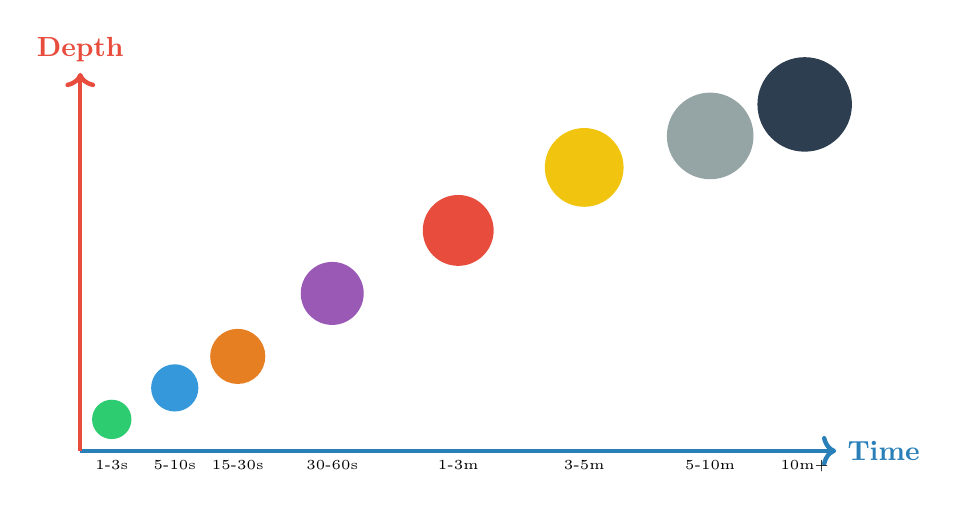
\begin{tikzpicture}[scale=0.8]
    \draw[ultra thick, ->, timingblue] (0,0) -- (12,0) node[right] {\textbf{Time}};
    \draw[ultra thick, ->, thoroughred] (0,0) -- (0,6) node[above] {\textbf{Depth}};
    
    % Plot verification methods
    \node[circle, fill=instantgreen, minimum size=0.5cm] at (0.5,0.5) {};
    \node[below] at (0.5,0) {\tiny 1-3s};
    
    \node[circle, fill=minimalblue, minimum size=0.6cm] at (1.5,1) {};
    \node[below] at (1.5,0) {\tiny 5-10s};
    
    \node[circle, fill=targetedorange, minimum size=0.7cm] at (2.5,1.5) {};
    \node[below] at (2.5,0) {\tiny 15-30s};
    
    \node[circle, fill=standardpurple, minimum size=0.8cm] at (4,2.5) {};
    \node[below] at (4,0) {\tiny 30-60s};
    
    \node[circle, fill=thoroughred, minimum size=0.9cm] at (6,3.5) {};
    \node[below] at (6,0) {\tiny 1-3m};
    
    \node[circle, fill=multimethod, minimum size=1cm] at (8,4.5) {};
    \node[below] at (8,0) {\tiny 3-5m};
    
    \node[circle, fill=completegray, minimum size=1.1cm] at (10,5) {};
    \node[below] at (10,0) {\tiny 5-10m};
    
    \node[circle, fill=formalblack, minimum size=1.2cm] at (11.5,5.5) {};
    \node[below] at (11.5,0) {\tiny 10m+};
\end{tikzpicture}
\end{center}

\tableofcontents
\newpage

% =============================
% EXECUTIVE SUMMARY
% =============================
\section{Executive Summary}

\begin{strategybox}{The Verification Spectrum}
Verification exists on a continuous spectrum from instant intuition to formal proof. The appropriate level depends on:
\begin{itemize}[nosep]
\item \textbf{Available time}: Competition vs. homework vs. research
\item \textbf{Problem difficulty}: Early-band vs. mid-band vs. late-band
\item \textbf{Confidence level}: High confidence needs less verification
\item \textbf{Cost of errors}: High-stakes situations need more verification
\item \textbf{Learning goals}: Deep understanding vs. quick solving
\end{itemize}
\end{strategybox}

\subsection{Quick Reference Matrix}

\begin{center}
\begin{tabularx}{\textwidth}{|>{\raggedright\arraybackslash}X|>{\raggedright\arraybackslash}X|>{\raggedright\arraybackslash}X|>{\raggedright\arraybackslash}X|>{\raggedright\arraybackslash}X|}
\hline
\textbf{Verification Level} & \textbf{Time} & \textbf{AMC12 Problems} & \textbf{Confidence Req.} & \textbf{Error Detection} \\
\hline
Instant Gut Check & 1-3s & 1-3 & 95\%+ & Major errors only \\
\hline
Minimal Sanity Check & 5-10s & 1-5 & 90\%+ & Magnitude/sign errors \\
\hline
Targeted Spot Check & 15-30s & 4-8 & 80\%+ & Key step errors \\
\hline
Standard Verification & 30-60s & 6-12 & 70\%+ & Most computational errors \\
\hline
Thorough Verification & 1-3m & 10-15 & 60\%+ & Logic and computation \\
\hline
Multi-Method & 3-5m & 13-18 & 50\%+ & Systematic errors \\
\hline
Complete Mathematical & 5-10m & 19-20 & 40\%+ & All error types \\
\hline
Formal Proof-Level & 10m+ & N/A & Any & Guarantees correctness \\
\hline
\end{tabularx}
\end{center}

\newpage

% =============================
% LEVEL 1: INSTANT GUT CHECK
% =============================
\section{Level 1: Instant Gut Check (1-3 seconds)}

\begin{instantbox}{Overview}
The fastest verification level based on intuition and pattern recognition. Your brain instantly recognizes when something "feels wrong" based on years of mathematical experience.
\end{instantbox}

\subsection{When to Use}
\begin{itemize}
\item Problems 1-3 in AMC12
\item Extremely high confidence (95\%+)
\item Simple computational problems
\item When you've seen similar problems many times
\item Time-critical situations with no room for detailed checks
\end{itemize}

\subsection{What It Catches}
\begin{itemize}
\item Answers that are obviously too large or too small
\item Wrong order of magnitude (100 instead of 10)
\item Negative when positive expected
\item Non-integer when integer required
\item Impossible probabilities (>1 or <0)
\end{itemize}

\begin{warningbox}{Limitations}
\begin{itemize}[nosep]
\item Won't catch subtle computational errors
\item Misses sign errors in intermediate steps
\item Can't verify logical reasoning
\item Unreliable for unfamiliar problem types
\end{itemize}
\end{warningbox}

\subsection{Example Application}

\begin{instantbox}{Problem: Find 20\% of 450}
\textbf{Solution}: $0.2 \times 450 = 90$

\textbf{Instant Check} (2 seconds):
\begin{itemize}[nosep]
\item "20\% is one-fifth"
\item "One-fifth of 450 is about 90"
\item "Feels right" \checkmark
\end{itemize}
\end{instantbox}

\newpage

% =============================
% LEVEL 2: MINIMAL/RAPID SANITY CHECK
% =============================
\section{Level 2: Minimal/Rapid Sanity Check (5-10 seconds)}

\begin{minimalbox}{Overview}
Quick verification focusing on the most common error types. This is the "quick magnitude check" mentioned in AMC12 strategy guides for early-band problems.
\end{minimalbox}

\subsection{Core Components}

\begin{minimalbox}{The 10-Second Checklist}
\begin{enumerate}[nosep]
\item \textbf{Magnitude Check}: Is the answer in the right ballpark?
\item \textbf{Units Check}: Are units correct and consistent?
\item \textbf{Sign Check}: Positive/negative as expected?
\item \textbf{Parity Check}: Even/odd if required?
\item \textbf{Boundary Check}: Within expected bounds?
\end{enumerate}
\end{minimalbox}

\subsection{Specific Techniques}

\subsubsection{Quick Magnitude Check}
\begin{itemize}
\item Round to nice numbers
\item Use benchmarks: $\pi \approx 3$, $\sqrt{2} \approx 1.4$, $e \approx 2.7$
\item Compare to known values
\item Check decimal point placement
\end{itemize}

\subsubsection{Units/Dimensional Check}
\begin{itemize}
\item Verify dimensions match (length vs. area vs. volume)
\item Check unit conversions
\item Ensure answer has required units
\end{itemize}

\subsubsection{Divisibility Quick Check}
\begin{itemize}
\item Last digit for divisibility by 2, 5, 10
\item Digit sum for divisibility by 3, 9
\item Quick mental division for small factors
\end{itemize}

\subsubsection{Answer-Choice Cross-Check (AMC12)}
\begin{itemize}
\item Eliminate options by units, sign, parity, and magnitude
\item Test modular residues (e.g., mod 3, 4, 9) when applicable
\item Plug candidate choices into key constraints to prune quickly
\end{itemize}

\begin{successbox}{AMC12 Application}
\begin{itemize}[nosep]
\item \problemrange{1-5}: Use as primary verification (90-95\% success)
\item \problemrange{6-10}: Use when confidence > 90\%
\item \textbf{Time saved}: 50-90 seconds vs. full verification
\item \textbf{Success rate}: Catches 80\% of major errors
\end{itemize}
\end{successbox}

\subsection{Example Application}

\begin{minimalbox}{Problem: A circle has area $36\pi$. Find its circumference.}
\textbf{Solution}: $A = \pi r^2 = 36\pi \Rightarrow r = 6 \Rightarrow C = 2\pi r = 12\pi$

\textbf{Minimal Check} (8 seconds):
\begin{itemize}[nosep]
\item Magnitude: "Radius 6, circumference about $6 \times 6 = 36$... wait, $2\pi \times 6 \approx 12 \times 3 = 36$" \checkmark
\item Units: "Area in square units, circumference in linear units" \checkmark
\item Sign: "Positive as expected" \checkmark
\item Reasonableness: "Circumference < area numerically for r = 6" \checkmark
\item General: For $r > 2$, $2\pi r < \pi r^2$
\end{itemize}
\end{minimalbox}

\newpage

% =============================
% LEVEL 3: TARGETED SPOT CHECK
% =============================
\section{Level 3: Targeted Spot Check (15-30 seconds)}

\begin{targetedbox}{Overview}
Strategic verification of the most error-prone parts of your solution. Focus on critical steps, tricky calculations, and common mistake points.
\end{targetedbox}

\subsection{What to Target}

\begin{targetedbox}{Priority Targets}
\begin{enumerate}
\item \textbf{The trickiest calculation}: Where you're most likely to make errors
\item \textbf{Sign changes}: Especially with inequalities
\item \textbf{Division steps}: Check for division by zero, sign preservation
\item \textbf{Substitution points}: Where you plug in values
\item \textbf{Final simplification}: Common location for arithmetic errors
\end{enumerate}
\end{targetedbox}

\subsection{Techniques}

\subsubsection{One-Point Test}
\begin{itemize}
\item Test with $n = 1$ or $x = 0$ if trivial
\item Check one boundary value
\item Verify one special case
\end{itemize}

\subsubsection{Critical Step Verification}
\begin{itemize}
\item Re-calculate the most complex step
\item Double-check the step you're least confident about
\item Verify the step with the most operations
\end{itemize}

\subsubsection{Endpoint Check}
\begin{itemize}
\item For optimization: check endpoints
\item For inequalities: check boundary cases
\item For sequences: check first and last terms
\end{itemize}

\begin{contextbox}{Competition Strategy}
\begin{itemize}[nosep]
\item \problemrange{6-10}: Primary verification method
\item \problemrange{11-15}: When time is limited
\item \textbf{Focus on}: Steps where you hesitated or erased
\item \textbf{Skip}: Steps you're 100\% confident about
\end{itemize}
\end{contextbox}

\subsection{Example Application}

\begin{targetedbox}{Problem: Solve $x^2 - 7x + 10 = 0$ for the sum of solutions}
\textbf{Solution}: By Vieta's formulas, sum = $-(-7)/1 = 7$

\textbf{Targeted Check} (20 seconds):
\begin{itemize}[nosep]
\item \textbf{Target}: Verify Vieta's formula application
\item Factor check: $(x-2)(x-5) = 0 \Rightarrow x = 2, 5$
\item Sum: $2 + 5 = 7$ \checkmark
\item \textbf{Skip}: Full expansion verification
\end{itemize}
\end{targetedbox}

\newpage

% =============================
% LEVEL 4: STANDARD VERIFICATION
% =============================
\section{Level 4: Standard Verification (30-60 seconds)}

\begin{standardbox}{Overview}
The traditional "check your work" approach. Substitute answers back, verify main calculations, and ensure all conditions are satisfied.
\end{standardbox}

\subsection{Core Components}

\begin{standardbox}{Standard Verification Protocol}
\begin{enumerate}
\item \textbf{Substitution Check}: Plug answer back into original equation
\item \textbf{Arithmetic Verification}: Check main computational steps
\item \textbf{Constraint Check}: Verify all given conditions are met
\item \textbf{Domain Check}: Ensure answer is in valid domain
\item \textbf{Extraneous Solutions}: Re-validate after squaring/absolute values/rationalizing
\item \textbf{Reasonableness Test}: Compare to estimated answer
\end{enumerate}
\end{standardbox}

\subsection{Techniques by Problem Type}

\subsubsection{Algebraic Problems}
\begin{itemize}
\item Substitute solution back into original equation
\item Verify factorization by expansion
\item Check discriminant for number of solutions
\item Exclude values that make denominators zero
\end{itemize}

\subsubsection{Geometric Problems}
\begin{itemize}
\item Verify angle sum properties
\item Check distance formulas
\item Confirm area/volume formulas used correctly
\item Ensure triangle inequality holds when inferring side lengths
\end{itemize}

\subsubsection{Word Problems}
\begin{itemize}
\item Check answer against problem context
\item Verify units throughout
\item Ensure answer is practical/realistic
\end{itemize}

\subsubsection{Probability Problems}
\begin{itemize}
\item Verify probabilities are in $[0,1]$ and totals sum to $1$
\item Ensure independence/conditional assumptions are correctly applied
\item Cross-check with complementary events when simpler
\end{itemize}

\subsubsection{Counting Problems}
\begin{itemize}
\item Guard against over/undercounting; use a simple double-count sanity check
\item Validate complements and totals match
\item Confirm handling of identical items and symmetry cases
\end{itemize}

\begin{successbox}{Effectiveness}
\begin{itemize}[nosep]
\item Catches 85-90\% of computational errors
\item Catches 70-80\% of conceptual errors
\item \problemrange{11-15}: Recommended minimum verification
\item Time investment yields high error detection rate
\end{itemize}
\end{successbox}

\subsection{Example Application}

\begin{standardbox}{Problem: Find all real $x$ where $\sqrt{x+3} + \sqrt{x-1} = 4$}
\textbf{Solution}: Square and solve to get $x = \frac{13}{4}$

\textbf{Standard Verification} (45 seconds):
\begin{enumerate}[nosep]
\item \textbf{Domain check}: $x \geq 1$ for both radicals, $\frac{13}{4} = 3.25 \geq 1$ \checkmark
\item \textbf{Substitution}: $\sqrt{3.25+3} + \sqrt{3.25-1} = \sqrt{6.25} + \sqrt{2.25} = 2.5 + 1.5 = 4$ \checkmark
\item \textbf{Arithmetic check}: Re-verify $6.25 = (2.5)^2$ and $2.25 = (1.5)^2$ \checkmark
\item \textbf{Reasonableness}: With domain $x \geq 1$ and from the squaring step $x \leq 7$, so $x \in [1,7]$ \checkmark
\end{enumerate}
\end{standardbox}

\newpage

% =============================
% LEVEL 5: THOROUGH VERIFICATION
% =============================
\section{Level 5: Thorough Verification (1-3 minutes)}

\begin{thoroughbox}{Overview}
Comprehensive checking of all major steps, multiple test cases, and verification of all mathematical properties. This level ensures high confidence in your solution.
\end{thoroughbox}

\subsection{Complete Checklist}

\begin{thoroughbox}{Thorough Verification Components}
\begin{enumerate}
\item \textbf{Step-by-step verification}: Check each major transformation
\item \textbf{Multiple test cases}: Try several specific values
\item \textbf{Boundary behavior}: Check limits and edge cases
\item \textbf{Necessary \& sufficient}: Verify both directions if applicable
\item \textbf{Alternative approach glimpse}: Quick mental check via different method
\item \textbf{Error analysis}: Identify where errors could have occurred
\end{enumerate}
\end{thoroughbox}

\subsection{Advanced Techniques}

\subsubsection{Limiting Behavior Analysis}
\begin{itemize}
\item As $x \to \infty$, does answer behave correctly?
\item As parameters approach 0, does answer simplify correctly?
\item Do discrete cases match continuous limits?
\end{itemize}

\subsubsection{Symmetry Verification}
\begin{itemize}
\item If problem has symmetry, does answer reflect it?
\item Check answer for invariance under expected transformations
\item Verify parity (even/odd) properties maintained
\end{itemize}

\subsubsection{Dimensional Analysis}
\begin{itemize}
\item Track units through every step
\item Verify dimensional consistency
\item Check scaling behavior
\end{itemize}

\begin{contextbox}{When to Use Thorough Verification}
\begin{itemize}[nosep]
\item \problemrange{13-17}: Standard approach
\item Problems you found challenging
\item When answer seems surprising
\item Before moving to next section in competition
\item When you have extra time
\end{itemize}
\end{contextbox}

\subsection{Example Application}

\begin{thoroughbox}{Problem: How many integer solutions to $x^2 + y^2 \leq 25$?}
\textbf{Solution}: Count lattice points in circle of radius 5, get 81

\textbf{Thorough Verification} (2 minutes):
\begin{enumerate}[nosep]
\item \textbf{Boundary check}: Points on circle: $(0,\pm5), (\pm5,0), (\pm3,\pm4), (\pm4,\pm3)$ = 12 points \checkmark
\item \textbf{Symmetry check}: Should be symmetric in 4 quadrants + axes + origin \checkmark
\item \textbf{Small case}: Radius 2: $(0,0), (\pm1,0), (0,\pm1), (\pm1,\pm1), (\pm2,0), (0,\pm2)$ = 13 points
\item \textbf{Direct enumeration}: Summing permitted $x$ for $y=-5,\ldots,5$ yields total $81$ \checkmark
\item \textbf{Parity}: Count should be odd (center point + symmetric pairs) \checkmark
\end{enumerate}
\end{thoroughbox}

\newpage

% =============================
% LEVEL 6: MULTI-METHOD VERIFICATION
% =============================
\section{Level 6: Multi-Method Verification (3-5 minutes)}

\begin{multimethodbox}{Overview}
Solve the problem using completely different approaches. When independent methods yield the same answer, confidence approaches certainty.
\end{multimethodbox}

\subsection{Method Combinations}

\begin{multimethodbox}{Common Multi-Method Approaches}
\begin{enumerate}
\item \textbf{Algebraic + Geometric}: Solve algebraically, verify with diagram
\item \textbf{Analytic + Synthetic}: Coordinates vs. pure geometry
\item \textbf{Direct + Indirect}: Forward solution vs. working backwards
\item \textbf{Exact + Approximate}: Precise calculation vs. estimation
\item \textbf{General + Special}: Formula vs. specific cases
\item \textbf{Theoretical + Computational}: Proof vs. calculation
\end{enumerate}
\end{multimethodbox}

\subsection{Problem-Specific Strategies}

\subsubsection{Optimization Problems}
\begin{itemize}
\item Method 1: Calculus (derivatives)
\item Method 2: Algebraic (complete the square)
\item Method 3: Geometric (visual inspection)
\end{itemize}

\subsubsection{Counting Problems}
\begin{itemize}
\item Method 1: Direct counting
\item Method 2: Complement counting
\item Method 3: Generating functions
\item Method 4: Recursion
\end{itemize}

\subsubsection{Geometric Problems}
\begin{itemize}
\item Method 1: Coordinate geometry
\item Method 2: Synthetic geometry
\item Method 3: Trigonometry
\item Method 4: Vector methods
\end{itemize}

\begin{successbox}{Benefits of Multi-Method Verification}
\begin{itemize}[nosep]
\item 95-99\% confidence in answer
\item Catches systematic errors in approach
\item Provides deeper understanding
\item Often reveals elegant solutions
\item Builds problem-solving flexibility
\end{itemize}
\end{successbox}

\subsection{Example Application}

\begin{multimethodbox}{Problem: Find area of triangle with vertices $(0,0)$, $(5,0)$, $(2,3)$}

\textbf{Method 1 - Formula} (30 seconds):
$$A = \frac{1}{2}|x_1(y_2-y_3) + x_2(y_3-y_1) + x_3(y_1-y_2)|$$
$$A = \frac{1}{2}|0(0-3) + 5(3-0) + 2(0-0)| = \frac{15}{2}$$

\textbf{Method 2 - Base × Height} (20 seconds):
Base = 5 (along x-axis), Height = 3 (y-coordinate)
$$A = \frac{1}{2} \times 5 \times 3 = \frac{15}{2}$$ \checkmark

\textbf{Method 3 - Vectors} (40 seconds):
$$\vec{v_1} = (5,0), \vec{v_2} = (2,3)$$
$$A = \frac{1}{2}||\vec{v_1} \times \vec{v_2}|| = \frac{1}{2}|5 \cdot 3 - 0 \cdot 2| = \frac{15}{2}$$ \checkmark
\end{multimethodbox}

\newpage

% =============================
% LEVEL 7: COMPLETE MATHEMATICAL VERIFICATION
% =============================
\section{Level 7: Complete Mathematical Verification (5-10 minutes)}

\begin{completebox}{Overview}
Full mathematical verification including proof of uniqueness, verification of all conditions, complete error analysis, and formal justification of every step.
\end{completebox}

\subsection{Components of Complete Verification}

\begin{completebox}{The Complete Verification Protocol}
\begin{enumerate}
\item \textbf{Existence}: Prove solution exists
\item \textbf{Uniqueness}: Prove solution is unique (if claimed)
\item \textbf{Necessity}: Show solution must satisfy all conditions
\item \textbf{Sufficiency}: Show conditions guarantee solution
\item \textbf{Completeness}: Verify all cases covered
\item \textbf{Consistency}: Check for contradictions
\item \textbf{Error bounds}: Quantify potential errors
\end{enumerate}
\end{completebox}

\subsection{Formal Verification Techniques}

\subsubsection{Proof by Contradiction}
\begin{itemize}
\item Assume answer is wrong
\item Derive contradiction
\item Conclude answer must be correct
\end{itemize}

\subsubsection{Inductive Verification}
\begin{itemize}
\item Verify base case
\item Verify inductive step
\item Confirm strong/weak induction appropriate
\end{itemize}

\subsubsection{Exhaustive Case Analysis}
\begin{itemize}
\item List all possible cases
\item Verify each case individually
\item Confirm cases are exhaustive and mutually exclusive
\end{itemize}

\begin{warningbox}{Time Management}
\begin{itemize}[nosep]
\item Rarely appropriate for competition settings
\item Reserve for \problemrange{19-20} if time permits
\item More suitable for homework/research
\item Can be overkill for simple problems
\end{itemize}
\end{warningbox}

\subsection{Example Application}

\begin{completebox}{Problem: Prove that $\sqrt{2}$ is irrational}

\textbf{Complete Verification}:

\textbf{1. Assumption}: Suppose $\sqrt{2} = \frac{p}{q}$ where $p,q \in \mathbb{Z}$, $\gcd(p,q) = 1$

\textbf{2. Derivation}: 
\begin{align}
2 &= \frac{p^2}{q^2}\\
2q^2 &= p^2\\
\therefore p^2 \text{ is even} &\Rightarrow p \text{ is even}\\
\text{Let } p = 2k &\Rightarrow 2q^2 = 4k^2\\
q^2 &= 2k^2\\
\therefore q^2 \text{ is even} &\Rightarrow q \text{ is even}
\end{align}

\textbf{3. Contradiction}: Both $p$ and $q$ are even, contradicting $\gcd(p,q) = 1$

\textbf{4. Conclusion}: $\sqrt{2}$ must be irrational \checkmark

\textbf{5. Error Analysis}: No computational errors, logic is sound

\textbf{6. Uniqueness}: N/A for existence proof
\end{completebox}

\newpage

% =============================
% LEVEL 8: FORMAL PROOF-LEVEL VERIFICATION
% =============================
\section{Level 8: Formal Proof-Level Verification (10+ minutes)}

\begin{formalbox}{Overview}
Rigorous mathematical proof with complete logical structure, formal notation, and verification of all axioms and theorems used. Publication-quality mathematics.
\end{formalbox}

\subsection{Formal Proof Components}

\begin{formalbox}{Elements of Formal Verification}
\begin{enumerate}
\item \textbf{Axiom verification}: Check all axioms invoked
\item \textbf{Theorem application}: Verify hypotheses of all theorems used
\item \textbf{Logical structure}: Formal symbolic logic if needed
\item \textbf{Definition checking}: Ensure all terms properly defined
\item \textbf{Quantifier analysis}: Verify $\forall$ and $\exists$ statements
\item \textbf{Edge case examination}: Check measure-zero sets, infinities
\item \textbf{Convergence proofs}: For limits and series
\end{enumerate}
\end{formalbox}

\subsection{Advanced Verification Methods}

\subsubsection{Computer-Assisted Proof}
\begin{itemize}
\item Formal verification systems (Coq, Lean, Isabelle)
\item Symbolic computation (Mathematica, Maple)
\item Automated theorem provers
\end{itemize}

\subsubsection{Peer Review Process}
\begin{itemize}
\item Independent verification by experts
\item Line-by-line proof checking
\item Verification of novel techniques
\end{itemize}

\begin{contextbox}{Appropriate Contexts}
\begin{itemize}[nosep]
\item Mathematical research papers
\item Thesis/dissertation work
\item Verifying famous conjectures
\item Creating new theorems
\item Never needed for AMC12
\end{itemize}
\end{contextbox}

\newpage

% =============================
% SPECIALIZED VERIFICATION METHODS
% =============================
\section{Specialized Verification Methods}

\begin{specializedbox}{Domain-Specific Techniques}
Different mathematical domains require specialized verification approaches tailored to their unique characteristics.
\end{specializedbox}

\subsection{Probabilistic Verification}

\begin{specializedbox}{Monte Carlo Verification}
\begin{itemize}
\item Generate random test cases
\item Compare statistical results to theoretical answer
\item Useful for: Probability problems, expected values
\item Confidence increases with sample size
\end{itemize}
\end{specializedbox}

\subsection{Geometric Verification}

\begin{specializedbox}{Construction Verification}
\begin{itemize}
\item Dynamic geometry software (GeoGebra, Desmos)
\item Verify constructions are possible
\item Check invariants under transformation
\item Visual confirmation of relationships
\end{itemize}
\end{specializedbox}

\subsection{Number Theory Verification}

\begin{specializedbox}{Modular Arithmetic Checks}
\begin{itemize}
\item Check answer modulo small primes
\item Verify divisibility properties
\item Use Chinese Remainder Theorem
\item Check quadratic residues
\end{itemize}
\end{specializedbox}

\subsection{Combinatorial Verification}

\begin{specializedbox}{Small Case Enumeration}
\begin{itemize}
\item Manually count small cases
\item Verify recurrence relations
\item Check generating function coefficients
\item Confirm bijections
\end{itemize}
\end{specializedbox}

\newpage

% =============================
% COMPETITION STRATEGY GUIDE
% =============================
\section{Competition Strategy Guide}

\begin{strategybox}{Optimal Verification by Problem Number}
Strategic verification allocation maximizes score while minimizing time investment.
\end{strategybox}

\subsection{Time-Optimal Verification Strategy}

\begin{center}
\begin{tabular}{|c|l|c|c|c|}
\hline
\textbf{Problems} & \textbf{Primary Method} & \textbf{Time} & \textbf{Backup Method} & \textbf{Success Rate} \\
\hline
1-3 & Instant Gut Check & 1-3s & Minimal Check & 95\%+ \\
4-5 & Minimal Sanity Check & 5-10s & Targeted Check & 92\%+ \\
6-8 & Targeted Spot Check & 15-30s & Standard & 88\%+ \\
9-12 & Standard Verification & 30-60s & Thorough & 85\%+ \\
13-15 & Thorough Verification & 1-3m & Multi-Method & 80\%+ \\
16-18 & Multi-Method & 3-5m & Complete & 75\%+ \\
19-20 & Complete (if time) & 5-10m & Multi-Method & 70\%+ \\
21-25 & Standard/Thorough & 1-3m & Skip if needed & 60\%+ \\
\hline
\end{tabular}
\end{center}

\subsection{Decision Flowchart}

\begin{center}
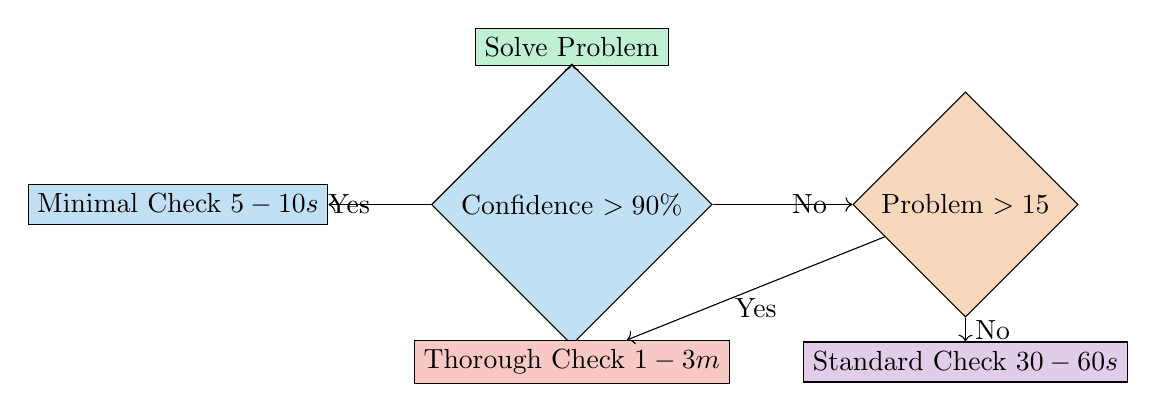
\begin{tikzpicture}[node distance=2cm]
    \node[draw, rectangle, fill=instantgreen!30] (start) {Solve Problem};
    \node[draw, diamond, fill=minimalblue!30, below of=start] (confidence) {Confidence $>90\%$};
    \node[draw, rectangle, fill=minimalblue!30, left of=confidence, xshift=-3cm] (minimal) {Minimal Check $5-10s$};
    \node[draw, diamond, fill=targetedorange!30, right of=confidence, xshift=3cm] (difficulty) {Problem $>15$};
    \node[draw, rectangle, fill=standardpurple!30, below of=difficulty] (standard) {Standard Check $30-60s$};
    \node[draw, rectangle, fill=thoroughred!30, below of=confidence] (thorough) {Thorough Check $1-3m$};
    
    \draw[->] (start) -- (confidence);
    \draw[->] (confidence) -- node[left] {Yes} (minimal);
    \draw[->] (confidence) -- node[right] {No} (difficulty);
    \draw[->] (difficulty) -- node[right] {No} (standard);
    \draw[->] (difficulty) -- node[below] {Yes} (thorough);
\end{tikzpicture}
\end{center}

\subsection{Time Management Guidelines}

\begin{strategybox}{The 75-Minute Plan}
\begin{itemize}[nosep]
\item \textbf{Problems 1-10} (20 min): Minimal verification only
\item \textbf{Problems 11-15} (20 min): Standard verification
\item \textbf{Problems 16-20} (25 min): Thorough verification
\item \textbf{Problems 21-25} (10 min): Best effort, skip verification if needed
\item \textbf{Review time}: Return to uncertain problems
\end{itemize}
\end{strategybox}

\newpage

% =============================
% COMMON PITFALLS AND WARNINGS
% =============================
\section{Common Pitfalls and Warnings}

\begin{warningbox}{Over-Verification Syndrome}
\textbf{Problem}: Spending too much time verifying easy problems\\
\textbf{Symptoms}: 
\begin{itemize}[nosep]
\item 5+ minutes on problems 1-5
\item Multi-method verification for high-confidence answers
\item Running out of time for later problems
\end{itemize}
\textbf{Solution}: Trust your instincts on early problems; save thorough checks for challenging ones
\end{warningbox}

\begin{warningbox}{Under-Verification Trap}
\textbf{Problem}: Insufficient verification leading to careless errors\\
\textbf{Symptoms}:
\begin{itemize}[nosep]
\item Arithmetic errors in final answers
\item Missing negative solutions
\item Forgetting to check domain restrictions
\end{itemize}
\textbf{Solution}: Minimum 10-second sanity check for ALL problems
\end{warningbox}

\begin{warningbox}{Verification Paralysis}
\textbf{Problem}: Getting stuck in verification loops\\
\textbf{Symptoms}:
\begin{itemize}[nosep]
\item Checking the same calculation 3+ times
\item Unable to move on despite correct answer
\item Anxiety about potential errors
\end{itemize}
\textbf{Solution}: Set hard time limits; trust systematic verification
\end{warningbox}

\subsection{Red Flags Requiring Extra Verification}

\begin{warningbox}{When to Upgrade Verification Level}
\begin{itemize}
\item Answer is not among the choices (double-check immediately)
\item Answer seems too simple for problem difficulty
\item You used a "clever trick" or shortcut
\item Problem involves many steps or complex algebra
\item Answer is negative when you expected positive
\item Answer is irrational when choices are rational
\item You're unsure about problem interpretation
\end{itemize}
\end{warningbox}

\newpage

% =============================
% PRACTICE EXERCISES
% =============================
\section{Practice Exercises}

\begin{strategybox}{Verification Training}
Practice identifying the appropriate verification level for different problem types and executing verification efficiently.
\end{strategybox}

\subsection{Exercise Set A: Choosing Verification Level}

For each problem, determine the appropriate verification level:

\begin{enumerate}
\item \textbf{Find 15\% of 80}
   \begin{itemize}[nosep]
   \item Recommended: Instant Gut Check (1-3s)
   \item Reasoning: Simple calculation, high confidence
   \end{itemize}

\item \textbf{Solve $x^3 - 6x^2 + 11x - 6 = 0$}
   \begin{itemize}[nosep]
   \item Recommended: Standard Verification (30-60s)
   \item Reasoning: Multiple roots, factoring required
   \end{itemize}

\item \textbf{Find the number of ways to arrange MATHEMATICS}
   \begin{itemize}[nosep]
   \item Recommended: Thorough Verification (1-3m)
   \item Reasoning: Complex counting with repetitions
   \end{itemize}

\item \textbf{Evaluate $\sin 30^\circ$}
   \begin{itemize}[nosep]
   \item Recommended: Instant Gut Check (1-3s)
   \item Reasoning: Standard value, memorized
   \end{itemize}

\item \textbf{Find area of triangle with vertices at $(1,2)$, $(4,6)$, $(7,2)$}
   \begin{itemize}[nosep]
   \item Recommended: Targeted Spot Check (15-30s)
   \item Reasoning: Formula application, check arithmetic
   \end{itemize}
\end{enumerate}

\subsection{Exercise Set B: Timed Verification Practice}

\begin{targetedbox}{15-Second Challenge}
Problem: If $f(x) = 2x + 3$ and $g(x) = x^2$, find $(f \circ g)(2)$

Solution: $(f \circ g)(2) = f(g(2)) = f(4) = 11$

Your 15-second verification:
\begin{itemize}[nosep]
\item $g(2) = 4$ \checkmark
\item $f(4) = 8 + 3 = 11$ \checkmark
\item Makes sense: composition of linear and quadratic \checkmark
\end{itemize}
\end{targetedbox}

\subsection{Exercise Set C: Multi-Method Practice}

\begin{multimethodbox}{Find Distance from $(3,4)$ to Line $x + y = 2$}

\textbf{Method 1 - Formula}:
$$d = \frac{|3 + 4 - 2|}{\sqrt{1^2 + 1^2}} = \frac{5}{\sqrt{2}} = \frac{5\sqrt{2}}{2}$$

\textbf{Method 2 - Perpendicular}:
\begin{itemize}[nosep]
\item Perpendicular from $(3,4)$ has slope 1
\item Line: $y - 4 = 1(x - 3) \Rightarrow y = x + 1$
\item Intersection: $x + 1 = 2 - x \Rightarrow x = \frac{1}{2}$
\item Distance: $\sqrt{(3-\frac{1}{2})^2 + (4-\frac{3}{2})^2} = \frac{5\sqrt{2}}{2}$ \checkmark
\end{itemize}
\end{multimethodbox}

\newpage

% =============================
% QUICK REFERENCE TABLES
% =============================
\section{Quick Reference Tables}

\subsection{Verification Method Selection Matrix}

\begin{center}
\begin{tabular}{|l|c|c|c|c|c|}
\hline
\textbf{Problem Type} & \textbf{Simple} & \textbf{Moderate} & \textbf{Complex} & \textbf{Novel} & \textbf{Proof} \\
\hline
Arithmetic & Instant & Minimal & Targeted & Standard & Thorough \\
Algebra & Minimal & Targeted & Standard & Thorough & Multi \\
Geometry & Minimal & Standard & Thorough & Multi & Complete \\
Counting & Targeted & Standard & Thorough & Multi & Complete \\
Number Theory & Targeted & Thorough & Multi & Complete & Formal \\
Calculus & Standard & Thorough & Multi & Complete & Formal \\
\hline
\end{tabular}
\end{center}

\subsection{Time Investment vs. Error Detection}

\noindent\small\textit{Note}: The percentages in this section are heuristic estimates intended to guide tradeoffs, not guarantees of actual performance.

\begin{center}
\begin{tabular}{|l|c|c|c|c|}
\hline
\textbf{Verification Level} & \textbf{Time} & \textbf{Major Errors} & \textbf{Minor Errors} & \textbf{Logic Errors} \\
\hline
Instant Gut Check & 1-3s & 60\% & 10\% & 5\% \\
Minimal Sanity Check & 5-10s & 80\% & 30\% & 10\% \\
Targeted Spot Check & 15-30s & 85\% & 50\% & 20\% \\
Standard Verification & 30-60s & 90\% & 70\% & 40\% \\
Thorough Verification & 1-3m & 95\% & 85\% & 60\% \\
Multi-Method & 3-5m & 98\% & 95\% & 80\% \\
Complete Mathematical & 5-10m & 99\% & 98\% & 95\% \\
Formal Proof-Level & 10m+ & 100\% & 100\% & 99\% \\
\hline
\end{tabular}
\end{center}

\subsection{Competition Score Impact}

\begin{center}
\begin{tabular}{|l|c|c|c|}
\hline
\textbf{Verification Strategy} & \textbf{Problems Attempted} & \textbf{Accuracy} & \textbf{Expected Score} \\
\hline
No verification & 20-25 & 70\% & 84-105 \\
Minimal only & 18-22 & 85\% & 91.8-112.2 \\
Balanced approach & 15-20 & 92\% & 82.8-110.4 \\
Over-verification & 12-15 & 98\% & 70.56-88.2 \\
\hline
\end{tabular}
\end{center}

\noindent\small\textit{Scoring note}: Table values assume 6 points per correct, 0 for wrong, 0 for omitted, to isolate the effect of verification. Values may be rounded for readability. For AMC12's current scoring (6 correct, 1.5 omitted, 0 wrong), add $1.5\times(25-\text{attempted})$ to each expected score.

\newpage

% =============================
% CONCLUSION
% =============================
\section{Conclusion}

\begin{strategybox}{Key Takeaways}
\begin{enumerate}
\item \textbf{Match verification to problem difficulty}: Don't over-verify easy problems
\item \textbf{Time is precious}: Every second counts in competition
\item \textbf{Trust your instincts}: High confidence requires less verification
\item \textbf{Know your weak points}: Extra verification where you commonly err
\item \textbf{Practice builds intuition}: Regular practice improves instant detection
\item \textbf{Flexibility is key}: Adapt verification level to time remaining
\end{enumerate}
\end{strategybox}

\subsection{The Verification Mastery Path}

\begin{center}
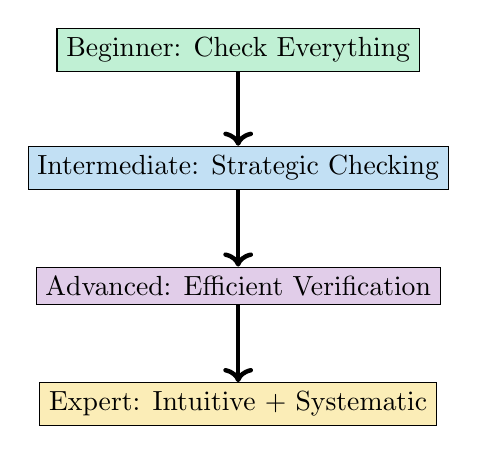
\begin{tikzpicture}[node distance=1.5cm]
    \node[draw, rectangle, fill=instantgreen!30, minimum width=3cm] (beginner) {Beginner: Check Everything};
    \node[draw, rectangle, fill=minimalblue!30, minimum width=3cm, below of=beginner] (intermediate) {Intermediate: Strategic Checking};
    \node[draw, rectangle, fill=standardpurple!30, minimum width=3cm, below of=intermediate] (advanced) {Advanced: Efficient Verification};
    \node[draw, rectangle, fill=multimethod!30, minimum width=3cm, below of=advanced] (expert) {Expert: Intuitive + Systematic};
    
    \draw[->, ultra thick] (beginner) -- (intermediate);
    \draw[->, ultra thick] (intermediate) -- (advanced);
    \draw[->, ultra thick] (advanced) -- (expert);
\end{tikzpicture}
\end{center}

\subsection{Final Recommendations}

\begin{successbox}{For Competition Success}
\begin{itemize}
\item \textbf{Problems 1-10}: Prioritize speed with minimal checks
\item \textbf{Problems 11-20}: Balance accuracy and time
\item \textbf{Problems 21-25}: Attempt if time permits, verify if very confident
\item \textbf{Review phase}: Return to flagged problems for deeper verification
\item \textbf{Never}: Spend more than 10\% of total time on verification
\item \textbf{Always}: Do at least a 5-second sanity check
\end{itemize}
\end{successbox}

\begin{contextbox}{Remember}
Perfect verification is not the goal—optimal verification is. The best verification strategy is one that maximizes your expected score given time constraints, not one that guarantees every answer is correct.
\end{contextbox}

\vfill

\begin{center}
\textit{Master the spectrum of verification, and you master the art of mathematical confidence.}
\end{center}

\end{document}